\documentclass[
	letterpaper, % Paper size, specify a4paper (A4) or letterpaper (US letter)
	10pt, % Default font size, specify 10pt, 11pt or 12pt
]{CSUniSchoolLabReport}

\usepackage{fancyvrb}
\usepackage{multicol}
\usepackage{subcaption}

\captionsetup[subfigure]{labelformat=empty}

\title{Calculating internal resistance of a battery.}

\author{Sebastien \textsc{Psarianos}\\ Sofiya \textsc{P'yavka}}

\date{\today}

\begin{document}

\maketitle

\begin{center}
	\begin{tabular}{l r}
		Date Performed: & October 6, 2022 \\
	\end{tabular}
\end{center}
\section{Introduction}
The primary objective of this experiment was to determine the internal resistance of a battery by comparing
the current and voltage readings across various resistors to readings from a power supply with approximately
$0$ internal resistance. The secondary objective of this experiment was to compare the results from the two
different Setups \textbf{Setup 1} and \textbf{Setup 2}.\\

All analysis was done with combination of Ohm's Law and Kirchoff's Loop Law.\\

\begin{tabular}{p{0.45\linewidth} p{0.45\linewidth}}
    $$\Delta V = IR$$
    -$\Delta V$ is the potential difference across a load\newline
    -$I$: The current through the load\newline
    -$R$: The resistance of the load
    \begin{center}
        \textbf{Equation 1: Ohm's Law}
    \end{center}
    &
    $$\Delta V_{loop} = \sum_i \Delta V_{load, i} = 0$$
    - $\Delta V_{load,i}$: Potential difference across $i$th load.
    \begin{center}
        \textbf{Equation 2: Kirchoff's Loop Law}
    \end{center}\\
    $$\Delta V_1 = \Delta V_2 = \Delta V_3 ...$$
    - $\Delta V_{i}$: Voltage drop along a parallel branch\newline
    All parallel branches have the same potential\newline
    difference.
    \begin{center}
        \textbf{Equation 3: Potential Difference across parallel branches}
    \end{center}
    &
    $$\sum_i I_{i, in} = \sum_j I_{j,out}$$
    - $I_{i, in}$: A current going into the junction\newline
    - $I_{j,out}$: A current coming out of the junction
    \begin{center}
        \textbf{Equation 4: Conservation of current in a junction}
    \end{center}

\end{tabular}

\section{Methods and Procedures}
\begin{figure}[H]
    \centering
	\begin{subfigure}{0.45\textwidth}
		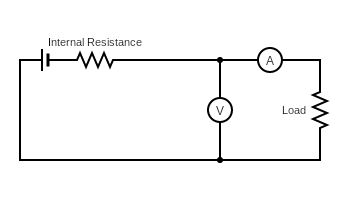
\includegraphics[width=\textwidth]{optionOne}
		\caption{\textbf{Setup 1}}
	\end{subfigure}
	\begin{subfigure}{0.45\textwidth}
		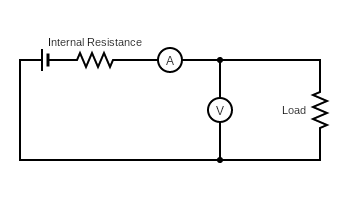
\includegraphics[width=\textwidth]{optionTwo}
		\caption{\textbf{Setup 2:}}
	\end{subfigure}
\end{figure}

In experiment 1, a circuit connected to a 6V battery as the power source was set up as shown in \textbf{Setup 1} using a voltmeter, an ammeter and a resistor. The voltmeter was set to a range of 30V and the ammeter was set to a range of 300mA. Note, the voltmeter and ammeter used were Keysight-U1272 multimeters. The current and the voltage across the power source were then measured and recorded. This was then repeated for seven more resistors all differing in resistance values. The same procedure was repeated, however, the setup of the circuit was modified as shown by \textbf{Setup 2}.\\

In experiment 2, a circuit connected to a power supply as the power source was set up as shown in \textbf{Setup 1} using a voltmeter, an ammeter and a resistor. Similarly, the voltmeter was set to a range of 30V and the ammeter was set to a range of 300mA. The power supply was set to 6.5V. The current and the voltage across the power source were then measured and recorded. This was then repeated seven more times using the same resistors in experiment 1. The same procedure was repeated, however, the setup of the circuit was modified as shown in \textbf{Setup 2}.  Furthermore, the entire procedure for both circuit setups was repeated for terminal voltage settings of 10V, 15V and 20V. \\

The range of resistor values that were used were chosen to provide a wide range of resistance values. The
resistance values ranged from $100\Omega\rightarrow 2800\Omega$. The reason n o resistors below $100\Omega$ were used was to prevent the amperage getting
too high and the resistor exhibiting overheating effects. As the resistance passed the range of $2800\Omega$ the
amperage values got quite small and were reaching the limits of the accuracy of the multimeter so $2800\Omega$
was chosen as an upper bound.\\

\section{Results}
Note, all curve fitting values and their uncertainties were calculated using the \lstinline{curve_fit} function from the \lstinline{scipy.optimize} module. All other referenced functions, equations and calculations can be found and are detailed in the Appendix section, in addition to the raw data and calculated uncertainties.\\

A linear model as defined by \textbf{Equation 5} was used to determine the output resistance of the power sources. The implementation of the model is shown by \textbf{Function 1} and was used for \lstinline{curve_fit}. The linear regression was performed on all raw data sets.\\

The uncertainties in the current and voltage readings were determined using \textbf{Equation 6}, implemented by \textbf{Function 2}. The equation itself was taken from the Keysight-U1272 manual for the multimeters. A detailed sample calculation for the uncertainties can be found under \textbf{Calculation 1 / 2}.\\

The graphs were then generated using \textbf{Function 3} which plots the experimental data and the line of best fit using the linear model and linear regression values determined by \lstinline{curve_fit}.\\

Note, all final resistance values were determined by multiplying the parameter of best fit for the resistance  determined by \lstinline{curve_fit} by 1000, as the current was measured in mA.\\

To determine the maximum current for each power supply setting, the x-intercept of the line of best fit was determined by rearranging \textbf{Equation 5} for the current when the voltage was equal to zero. Then the best fit parameters for each power supply setting were passed into the equation. The final value was multiplied by 1000 in order to determine the maximum current in amps rather than milliamps. This was done for the data collected from both experimental setups. The maximum currents and terminal voltages (determined from \lstinline{curve_fit}) were then plotted. The uncertainties for the terminal voltages were determined using \lstinline{curve_fit} and the uncertainties for the maximum current were determined using \textbf{Equation 7}.
\newpage
{\large\textbf{Graphs}}
\begin{figure}[H]
    \centering
	\begin{subfigure}{0.45\textwidth}
		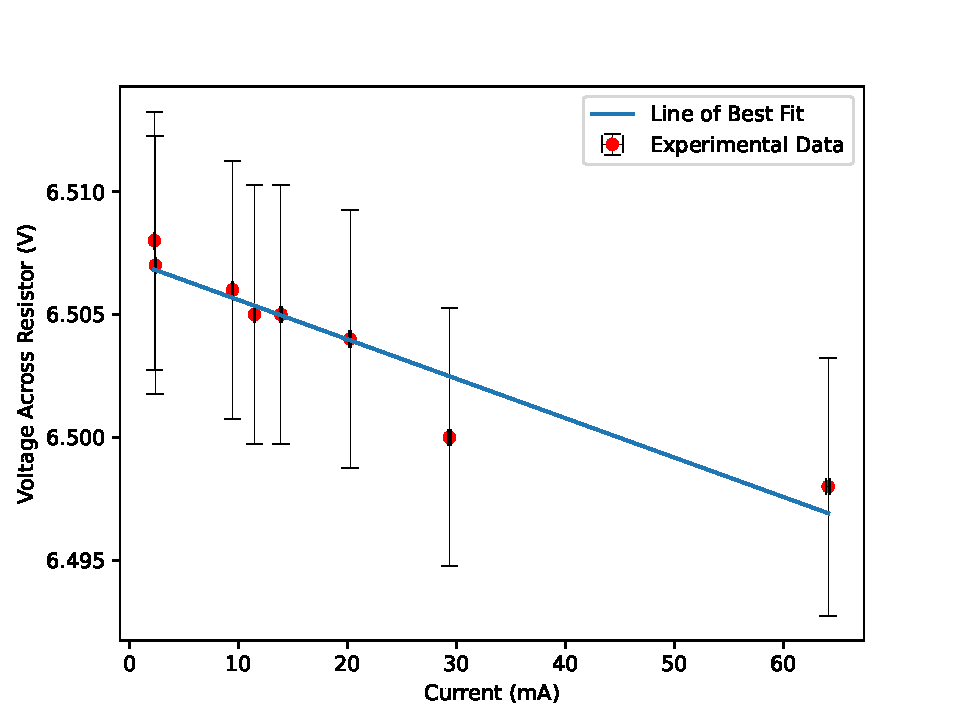
\includegraphics[width=\textwidth]{graph1}
		\caption{\textbf{Figure 3: Measured Voltage vs Measured Current for the circuit denoted in setup 1. The current and voltage measurements are taken at the locations of the respective detector in the schematic. The voltage source is the battery. The negative of the slope is the output resistance value.}}
	\end{subfigure}
    \hspace{0.08\textwidth}
	\begin{subfigure}{0.45\textwidth}
		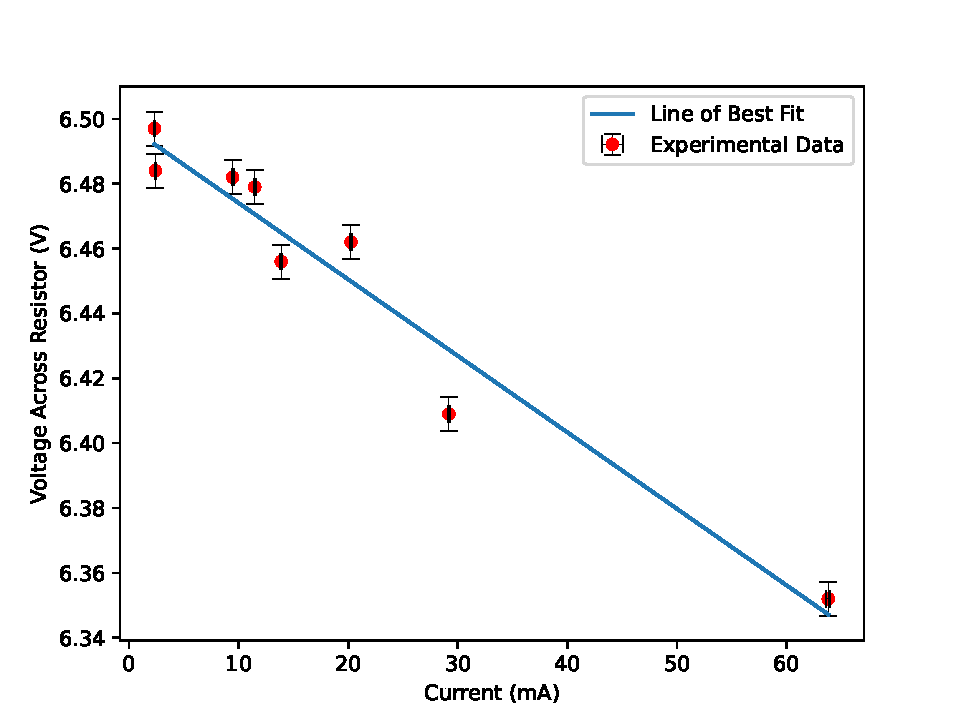
\includegraphics[width=\textwidth]{graph2}
		\caption{\textbf{Figure 2: Measured Voltage vs Measured Current for the circuit denoted in setup 2. The current and voltage measurements are taken at the locations of the respective detector in the schematic. The voltage source is the battery. The negative of the slope is the output resistance value.}}
	\end{subfigure}
    \begin{subfigure}{0.45\textwidth}
		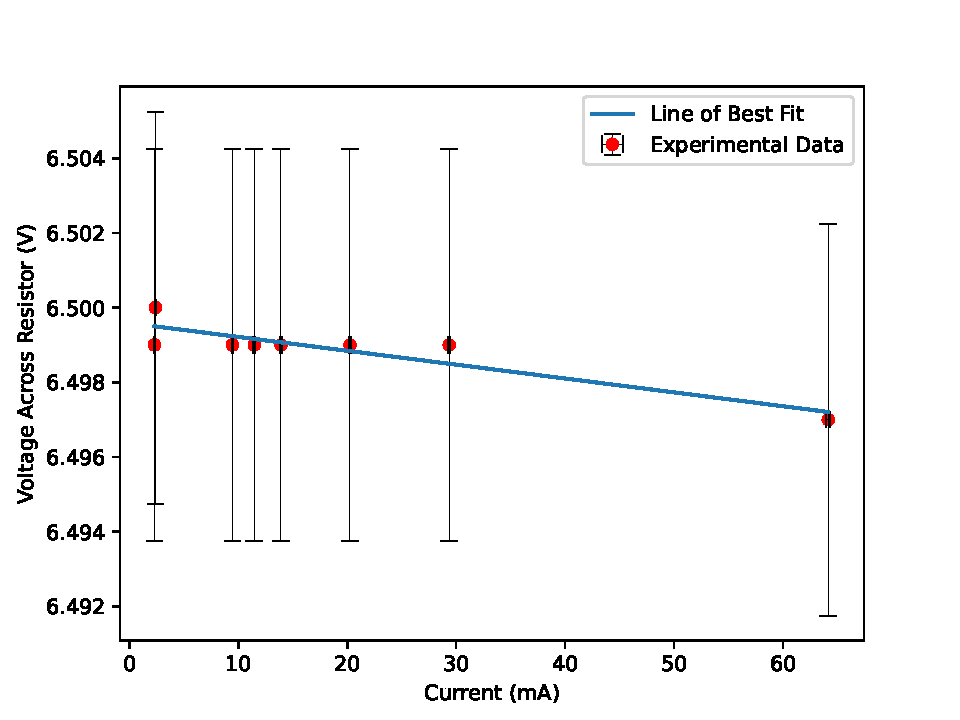
\includegraphics[width=\textwidth]{graph3}
		\caption{\textbf{Figure 3: Measured Voltage vs Measured Current for the circuit denoted in setup 1. The current and voltage measurements are taken at the locations of the respective detector in the schematic. The voltage source is the regulated power supply set at 6.5V. The negative of the slope is the output resistance value.}}
	\end{subfigure}
    \hspace{0.08\textwidth}
	\begin{subfigure}{0.45\textwidth}
		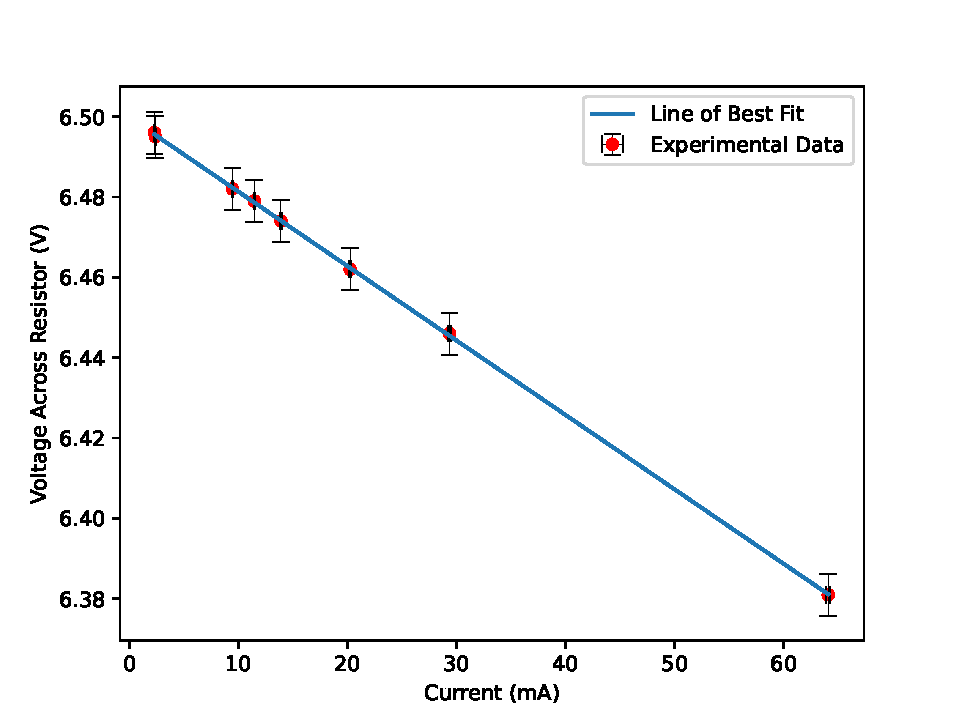
\includegraphics[width=\textwidth]{graph4}
		\caption{\textbf{Figure 4: Measured Voltage vs Measured Current for the circuit denoted in setup 2. The current and voltage measurements are taken at the locations of the respective detector in the schematic. The voltage source is the regulated power supply set at 6.5V. The negative of the slope is the output resistance value.}}
	\end{subfigure}

\end{figure}

\begin{figure}[H]
    \centering
    \begin{subfigure}{0.45\textwidth}
		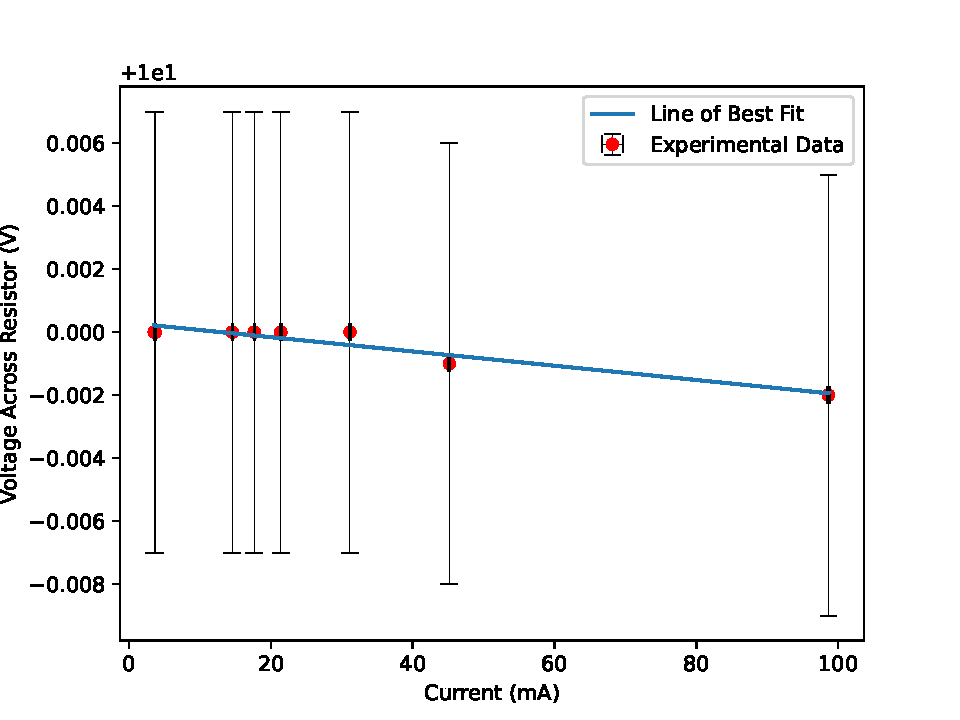
\includegraphics[width=\textwidth]{graph5}
		\caption{\textbf{Figure 5: Measured Voltage vs Measured Current for the circuit denoted in setup 1. The current and voltage measurements are taken at the locations of the respective detector in the schematic. The voltage source is the regulated power supply set at 10V. The negative of the slope is the output resistance value.}}
	\end{subfigure}
    \hspace{0.08\textwidth}
	\begin{subfigure}{0.45\textwidth}
		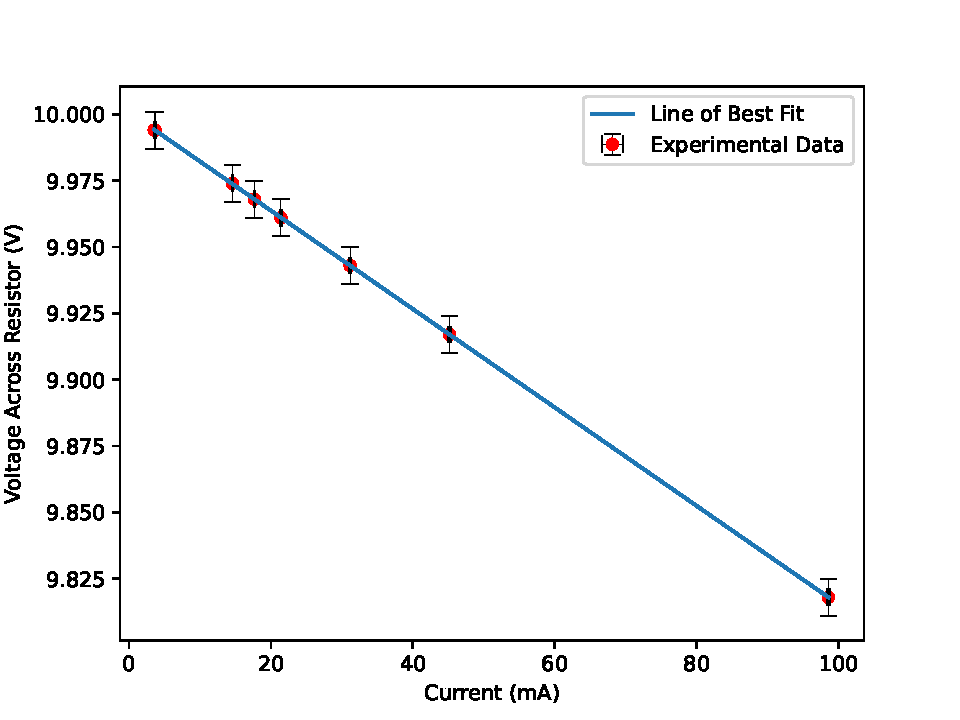
\includegraphics[width=\textwidth]{graph6}
		\caption{\textbf{Figure 6: Measured Voltage vs Measured Current for the circuit denoted in setup 2. The current and voltage measurements are taken at the locations of the respective detector in the schematic. The voltage source is the regulated power supply set at 10V. The negative of the slope is the output resistance value.}}
	\end{subfigure}
    \begin{subfigure}{0.45\textwidth}
		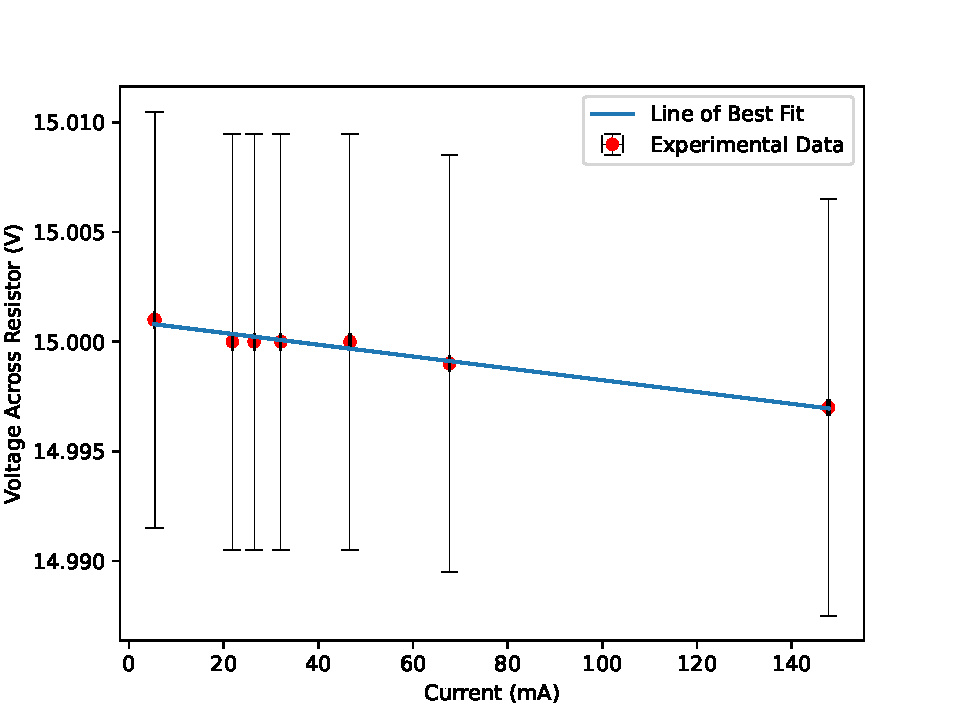
\includegraphics[width=\textwidth]{graph7}
		\caption{\textbf{Figure 7: Measured Voltage vs Measured Current for the circuit denoted in setup 1. The current and voltage measurements are taken at the locations of the respective detector in the schematic. The voltage source is the regulated power supply set at 15V. The negative of the slope is the output resistance value.}}
	\end{subfigure}
    \hspace{0.08\textwidth}
	\begin{subfigure}{0.45\textwidth}
		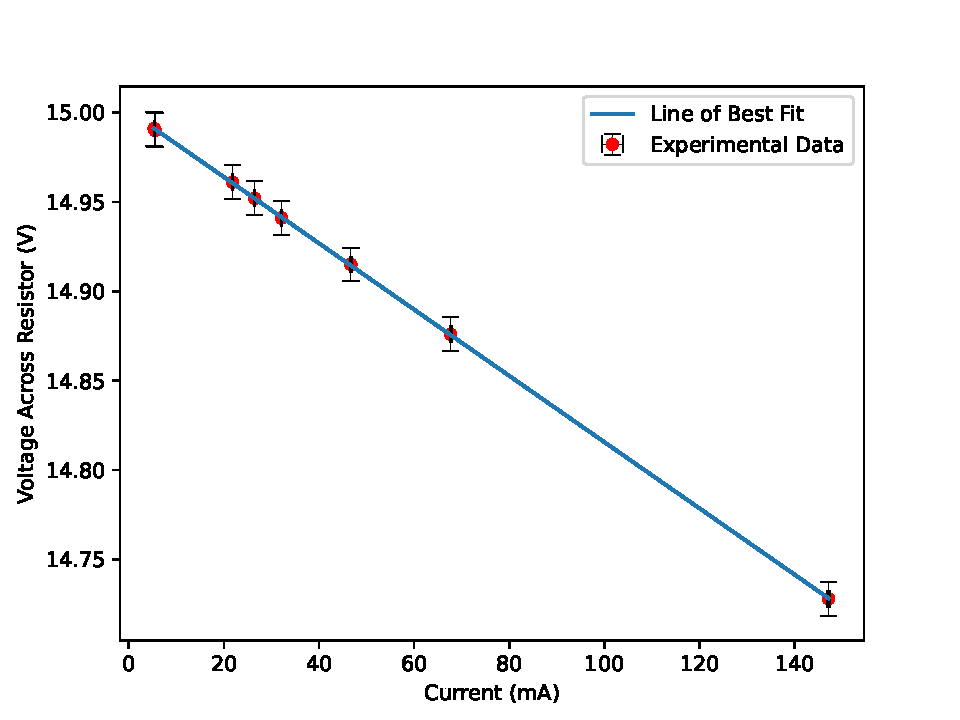
\includegraphics[width=\textwidth]{graph8}
		\caption{\textbf{Figure 8: Measured Voltage vs Measured Current for the circuit denoted in setup 2. The current and voltage measurements are taken at the locations of the respective detector in the schematic. The voltage source is the regulated power supply set at 15V. The negative of the slope is the output resistance value.}}
	\end{subfigure}
\end{figure}

\begin{figure}[H]
	\begin{subfigure}{0.45\textwidth}
		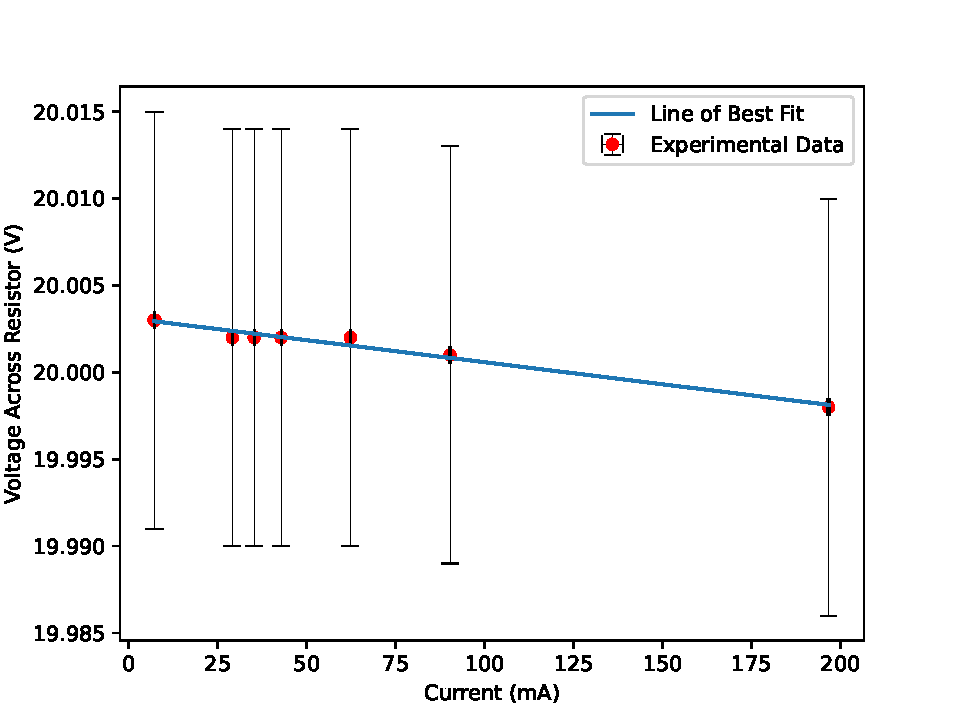
\includegraphics[width=\textwidth]{graph9}
		\caption{\textbf{Figure 9: Measured Voltage vs Measured Current for the circuit denoted in setup 1. The current and voltage measurements are taken at the locations of the respective detector in the schematic. The voltage source is the regulated power supply set at 20V. The negative of the slope is the output resistance value.}}
	\end{subfigure}
    \hspace{0.08\textwidth}
	\begin{subfigure}{0.45\textwidth}
		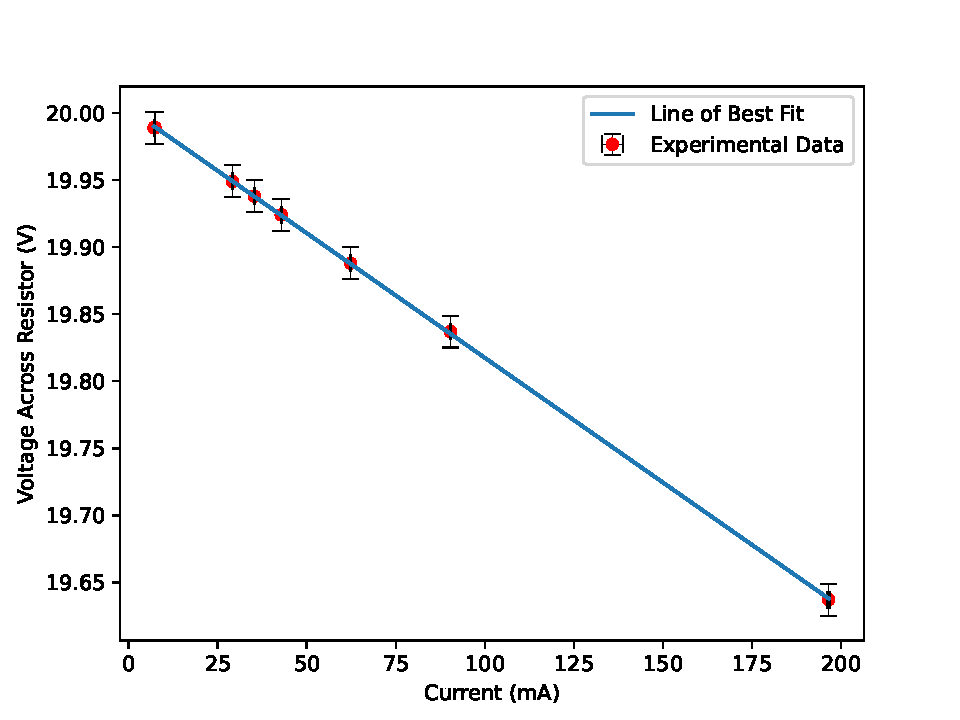
\includegraphics[width=\textwidth]{graph10}
		\caption{\textbf{Figure 10: Measured Voltage vs Measured Current for the circuit denoted in setup 2. The current and voltage measurements are taken at the locations of the respective detector in the schematic. The voltage source is the regulated power supply set at 20V. The negative of the slope is the output resistance value.}}
	\end{subfigure}
    \begin{subfigure}{0.45\textwidth}
		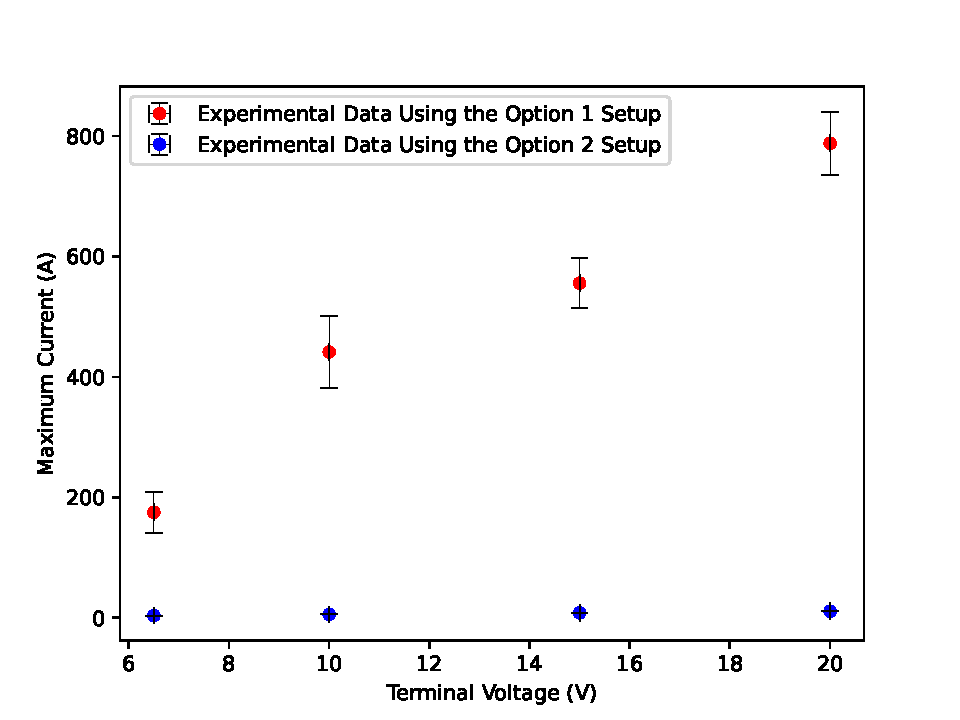
\includegraphics[width=\textwidth]{maxCurrent}
		\caption{\textbf{Figure 11: Graph demonstrating the relationship between maximum current and terminal voltage, varying linearly on one another.}}
	\end{subfigure}
\end{figure}

\newpage
\section{Analysis}
In experiment 1, the output resistance determined for the battery in \textbf{Setups 1 and 2} were $ 0.16 \pm 0.02 \Omega $ and $ 2.4 \pm 0.2 \Omega $ respectively. The negative of the slope of the line of best fit in \textbf{Graphs 1 and 2} represents the value of output resistance.

In experiment 2, the output resistance determined for the power supply for settings $6.5V$, $10V$, $15V$ and $20V$ in \textbf{Setup 1} were $ 0.037 \pm 0.007 \Omega $, $ 0.023 \pm 0.003 \Omega $, $ 0.027 \pm 0.002 \Omega $ and $ 0.025 \pm 0.002 \Omega $ respectively. The output resistance determined for the power supply for settings $6.5V$, $10V$, $15V$ and $20V$ in \textbf{Setup 2} were $ 1.853 \pm 0.008 \Omega $, $ 1.854 \pm 0.002 \Omega $, $ 1.853 \pm 0.004 \Omega $, $ 1.859 \pm 0.006 \Omega $ respectively. The negative of the slope of the line of best fit in \textbf{Graphs 3-10} represents the value of output resistance. In both setups, the value of the output resistance remains relatively consistent for all settings of voltage.

The experimental data plotted in all graphs demonstrate a linear dependence, verifying the relationship described by \textbf{Equation 8}.

Examining \textbf{Graph 11}, the maximum current approximately varies linearly with the terminal voltage. So as the terminal voltage increases, the maximum current increases proportionally. The internal electronics of the power supply ensure that the resistance is as minimal as possible so the output resistance approaches zero beyond the regulation regime.
\newpage
\section{Discussion}
Two main assumptions were made in the analysis of this experiment, namely that the voltmeter and
ammeter were both ideal. Ideal voltmeters have a resistance of $\infty$ and ideal ammeters have $0$ resistance. However,
in the real world, this is not possible.\\

The voltmeter in \textbf{Setup 1} was measuring the potential difference across the load and the ammeter,
whereas the voltmeter in \textbf{Setup 2} was measuring the potential difference across only the load. This
is reflected in the data, where the voltmeter measurements are consistently higher in the \textbf{Setup 1}
data. Since the voltmeter measurements were affected by the location of the ammeter, the ammeter had
a measurable effect on the circuit. For this to be the case it must have had some resistance. An ideal ammeter
would not affect any measurements no matter where it was placed. \\

By \textbf{Equation 3}, parallel branches in a circuit both have the same potential
difference. This means that there is a non-zero voltage drop in the voltmeter branch. By ohm's law:
$\Delta V_{vm} = I_{vm} R_{vm}, \ \Delta V_{vm} \ne 0 \implies I_{vm} \ne 0$. Where $vm$ denotes the voltmeter.\\

By conservation of charge \textbf{Equation 4}, the current through both branches must add up to the current through the battery. Therefore: $I_{batt} = I_{vm} + I_{load}$.\\

In \textbf{Setup 1}, the ammeter was placed on the load branch and is measuring $I_{load}$. In \textbf{Setup 2} the
ammeter was placed next to the battery, therefore it was reading the $I_{batt}$ value. The
purpose of the experiment was to calculate the internal resistance of the battery and the $I_{batt}$ value is much more useful in this
calculation. If the experiment was performed with only \textbf{Setup 1}, the $I_{batt}$ value could only be indirectly calculated and
not measured. Since $I_{batt} = I_{vm} +I_{load}$, $I_{vm}$ could be roughly estimated for each resistance by
subtracting measured ammeter values in \textbf{Setup 1} from measured values in \textbf{Setup 2}.   \\

If both the ammeter and the voltmeter were ideal, then both \textbf{Setups 1 and 2} would give identical
results. However, this was not the case so \textbf{Setup 2} was the superior setup for the objectives of this
experiment due to the fact that it was measuring the current that was needed for the calculations.\\

During the experiment, when the resistors on the lower end of the resistance range were measured
(specifically the $100\Omega$ and $200\Omega$ measurements), the current measurements would drop rapidly. This was likely
due to the resistor heating up. Although the lower end of the range was chosen to prevent this from
occurring, it would likely be a better idea for future experiments to do fewer measurements with low ohm resistors.
\newpage
\section{Appendix}

{\large\textbf{Equations}}\\

\begin{tabular}{p{0.45\linewidth} p{0.45\linewidth}}
    $$\Delta V = IR$$
    -$\Delta V$ is the potential difference across a load\newline
    -$I$: The current through the load\newline
    -$R$: The resistance of the load
    \begin{center}
        \textbf{Equation 1: Ohm's Law}
    \end{center}
    &
    $$\Delta V_{loop} = \sum_i \Delta V_{load, i} = 0$$
    - $\Delta V_{load,i}$: Potential difference across $i$th load.
    \begin{center}
        \textbf{Equation 2: Kirchoff's Loop Law}
    \end{center}\\
    $$\Delta V_1 = \Delta V_2 = \Delta V_3 ...$$
    - $\Delta V_{i}$: Voltage drop along a parallel branch\newline
    All parallel branches have the same potential\newline
    difference.
    \begin{center}
        \textbf{Equation 3: Potential Difference across parallel branches}
    \end{center}
    &
    $$\sum_i I_{i, in} = \sum_j I_{j,out}$$
    - $I_{i, in}$: A current going into the junction\newline
    - $I_{j,out}$: A current coming out of the junction
    \begin{center}
        \textbf{Equation 4: Conservation of current in a junction}
    \end{center}\\
    $$f(x) = b-ax$$
    \begin{center}
        \textbf{Equation 5: Linear Model}
    \end{center}
    &
    $$ u(x) = \pm\left|\frac{xp}{100} + c r\right|$$
    \begin{center}
        \textbf{Equation 6: Uncertainty calculation formula from multimeter manual}
    \end{center}\\
    $$ u\left(\frac{x}{y}\right) = \sqrt{\frac{u(x)}{x}^2 + \frac{u(y)}{y}^2}$$
    \begin{center}
        \textbf{Equation 7: Division error propagation}
    \end{center}
    &
    $$V = V_\infty - R_{int}I$$
    \begin{center}
        \textbf{Equation 8: Effect of internal resistance on output voltage}
    \end{center}
\end{tabular}\\\\
\newpage
{\large\textbf{Functions}}\\

\begin{verbatim}
    def linear(current, open_voltage, resistance):
        return open_voltage - resistance * current
    \end{verbatim}
\begin{center}
    \textbf{Function 1: Linear model (implements Equation 5)}
\end{center}

\begin{verbatim}
def calculate_uncertainty(value, res, percentage, multiplier):
    return value * percentage / 100 + res * multiplier
\end{verbatim}
\begin{center}
    \textbf{Function 2: Uncertainty calculation (implements Equation 6)}
\end{center}

\begin{verbatim}
def division_propagation(
    value_1, uncertainty_1, value_2, uncertainty_2, value_3
):
    return value_3 * np.sqrt(
        (uncertainty_1 / value_1) ** 2 + (uncertainty_2 / value_2) ** 2
    )
\end{verbatim}
\begin{center}
    \textbf{Function 3: Division Error propagation (implements Equation 7)}
\end{center}

{\large\textbf{Sample Calculations}}\\

This calculation is based on \textbf{Equation 6}\\
$r = 0.001$, $p = 0.05$, $c=2$ (from the Keysight manual)\\
Let $V_i$ represent an arbitrary voltage measurement made with the $30V$ setting.\\
$$u(V_i) = \pm \left|\frac{0.05V_i }{100} +  2* 0.001\right|V = \pm\left|0.0005V_i + 0.002\right|V$$
For example in table, the first measured voltage was: $V_1=6.498V$\\
$$u(V_1) = u(6.498V) = \pm \left|0.0005 \times 6.498 + 0.002\right|V \approx \pm 0.0052V$$
\begin{center}
    \textbf{Calculation 1: Voltmeter Calculation sample for $30V$ setting}\\

\end{center}

\vspace{10pt}
These calculations are based on \textbf{Equation 6}:\\
$r = 0.01$, $p = 0.2$, $c=5$ (from the Keysight manual)\\
Let $I_i$ represent an arbitrary current measurement made with the $300mA$ setting.\\
$$u(I_i) = \pm \left|\frac{0.2I_i }{100} +  5* 0.01\right|mA = \pm\left|0.002I_i + 0.05\right|mA$$
For example in table one, the first measured current was: $I_1 = 64.12mA$.
$$u(I_1)= u(64.12mA) = \pm\left|0.002 \times 64.12 + 0.05\right|mA \approx \pm 0.18mA$$
\begin{center}
    \textbf{Calculation 2: Ammeter Calculation sample for $300mA$ setting}
\end{center}

\textbf{Table Section} \\

\begin{tabular}{| p{0.14\textwidth} | p{0.14\textwidth} | p{0.14\textwidth} |}
    \hline
    Resistance ($\Omega$) & Voltage ($V$) & Current ($mA$)
    \hline    100 & 6.498 \pm 0.005249 & 6.498 \pm 0.17824\\
    220 & 6.5 \pm 0.00525 & 6.5 \pm 0.10874\\
    320 & 6.504 \pm 0.005252 & 6.504 \pm 0.09052000000000002\\
    470 & 6.505 \pm 0.0052525 & 6.505 \pm 0.07784\\
    570 & 6.505 \pm 0.0052525 & 6.505 \pm 0.07296\\
    690 & 6.506 \pm 0.005253000000000001 & 6.506 \pm 0.06894\\
    2700 & 6.507 \pm 0.0052535 & 6.507 \pm 0.05478\\
    2800 & 6.508 \pm 0.005254 & 6.508 \pm 0.05462\\
    \hline 
 \end{tabular}

\begin{tabular}{| p{0.14\textwidth} | p{0.14\textwidth} | p{0.14\textwidth} |}
    \hline
    Resistance ($\Omega$) & Voltage ($V$) & Current ($mA$)
    \hline    100 & 6.352 \pm 0.005176 & 6.352 \pm 0.17764000000000002\\
    220 & 6.409 \pm 0.005204500000000001 & 6.409 \pm 0.10838\\
    320 & 6.462 \pm 0.0052309999999999995 & 6.462 \pm 0.0905\\
    470 & 6.456 \pm 0.005228 & 6.456 \pm 0.07776000000000001\\
    570 & 6.479 \pm 0.0052395 & 6.479 \pm 0.07294\\
    690 & 6.482 \pm 0.005241000000000001 & 6.482 \pm 0.06892000000000001\\
    2700 & 6.484 \pm 0.005242 & 6.484 \pm 0.05478\\
    2800 & 6.497 \pm 0.0052485 & 6.497 \pm 0.05462\\
    \hline 
 \end{tabular}

\begin{tabular}{| p{0.14\textwidth} | p{0.14\textwidth} | p{0.14\textwidth} |}
    \hline
    Resistance ($\Omega$) & Voltage ($V$) & Current ($mA$)
    \hline    100 & 6.497 \pm 0.0052485 & 6.497 \pm 0.17832000000000003\\
    220 & 6.499 \pm 0.005249500000000001 & 6.499 \pm 0.10872000000000001\\
    320 & 6.499 \pm 0.005249500000000001 & 6.499 \pm 0.0905\\
    470 & 6.499 \pm 0.005249500000000001 & 6.499 \pm 0.07782\\
    570 & 6.499 \pm 0.005249500000000001 & 6.499 \pm 0.07294\\
    690 & 6.499 \pm 0.005249500000000001 & 6.499 \pm 0.06892000000000001\\
    2700 & 6.5 \pm 0.00525 & 6.5 \pm 0.05478\\
    2800 & 6.499 \pm 0.005249500000000001 & 6.499 \pm 0.0546\\
    \hline 
 \end{tabular}

\begin{tabular}{| p{0.14\textwidth} | p{0.14\textwidth} | p{0.14\textwidth} |}
    \hline
    Resistance ($\Omega$) & Voltage ($V$) & Current ($mA$)
    \hline    100 & 6.381 \pm 0.005190500000000001 & 6.381 \pm 0.17818\\
    220 & 6.446 \pm 0.005223 & 6.446 \pm 0.10872000000000001\\
    320 & 6.462 \pm 0.0052309999999999995 & 6.462 \pm 0.0905\\
    470 & 6.474 \pm 0.005237 & 6.474 \pm 0.07782\\
    570 & 6.479 \pm 0.0052395 & 6.479 \pm 0.07294\\
    690 & 6.482 \pm 0.005241000000000001 & 6.482 \pm 0.06892000000000001\\
    2700 & 6.495 \pm 0.0052475 & 6.495 \pm 0.05478\\
    2800 & 6.496 \pm 0.005248000000000001 & 6.496 \pm 0.05462\\
    \hline 
 \end{tabular}

\begin{tabular}{| p{0.14\textwidth} | p{0.14\textwidth} | p{0.14\textwidth} |}
    \hline
    Resistance ($\Omega$) & Voltage ($V$) & Current ($mA$)
    \hline    100 & 9.998 \pm 0.006999 & 9.998 \pm 0.24730000000000002\\
    220 & 9.999 \pm 0.0069995000000000005 & 9.999 \pm 0.14034000000000002\\
    320 & 10.0 \pm 0.007 & 10.0 \pm 0.11232\\
    470 & 10.0 \pm 0.007 & 10.0 \pm 0.09282\\
    570 & 10.0 \pm 0.007 & 10.0 \pm 0.0853\\
    690 & 10.0 \pm 0.007 & 10.0 \pm 0.07912000000000001\\
    2700 & 10.0 \pm 0.007 & 10.0 \pm 0.05736\\
    2800 & 10.0 \pm 0.007 & 10.0 \pm 0.057100000000000005\\
    \hline 
 \end{tabular}

\begin{tabular}{| p{0.14\textwidth} | p{0.14\textwidth} | p{0.14\textwidth} |}
    \hline
    Resistance ($\Omega$) & Voltage ($V$) & Current ($mA$)
    \hline    100 & 9.818 \pm 0.006909 & 9.818 \pm 0.24716\\
    220 & 9.917 \pm 0.0069585 & 9.917 \pm 0.14034000000000002\\
    320 & 9.943 \pm 0.0069715 & 9.943 \pm 0.11230000000000001\\
    470 & 9.961 \pm 0.006980500000000001 & 9.961 \pm 0.09282\\
    570 & 9.968 \pm 0.006984 & 9.968 \pm 0.0853\\
    690 & 9.974 \pm 0.006987 & 9.974 \pm 0.07912000000000001\\
    2700 & 9.994 \pm 0.006997000000000001 & 9.994 \pm 0.05736\\
    2800 & 9.994 \pm 0.006997000000000001 & 9.994 \pm 0.057100000000000005\\
    \hline 
 \end{tabular}

\begin{tabular}{| p{0.14\textwidth} | p{0.14\textwidth} | p{0.14\textwidth} |}
    \hline
    Resistance ($\Omega$) & Voltage ($V$) & Current ($mA$)
    \hline    100 & 14.997 \pm 0.0094985 & 14.997 \pm 0.3456\\
    220 & 14.999 \pm 0.009499500000000001 & 14.999 \pm 0.18544\\
    320 & 15.0 \pm 0.0095 & 15.0 \pm 0.14342\\
    470 & 15.0 \pm 0.0095 & 15.0 \pm 0.11424\\
    570 & 15.0 \pm 0.0095 & 15.0 \pm 0.10292000000000001\\
    690 & 15.0 \pm 0.0095 & 15.0 \pm 0.09368000000000001\\
    2700 & 15.001 \pm 0.0095005 & 15.001 \pm 0.06106\\
    2800 & 15.001 \pm 0.0095005 & 15.001 \pm 0.060660000000000006\\
    \hline 
 \end{tabular}

\begin{tabular}{| p{0.14\textwidth} | p{0.14\textwidth} | p{0.14\textwidth} |}
    \hline
    Resistance ($\Omega$) & Voltage ($V$) & Current ($mA$)
    \hline    100 & 14.728 \pm 0.009364 & 14.728 \pm 0.3443\\
    220 & 14.876 \pm 0.009438 & 14.876 \pm 0.18536000000000002\\
    320 & 14.915 \pm 0.0094575 & 14.915 \pm 0.14340000000000003\\
    470 & 14.941 \pm 0.009470500000000001 & 14.941 \pm 0.11422\\
    570 & 14.952 \pm 0.009476 & 14.952 \pm 0.10294\\
    690 & 14.961 \pm 0.009480500000000001 & 14.961 \pm 0.09368000000000001\\
    2700 & 14.99 \pm 0.009495 & 14.99 \pm 0.06106\\
    2800 & 14.991 \pm 0.0094955 & 14.991 \pm 0.060660000000000006\\
    \hline 
 \end{tabular}

\begin{tabular}{| p{0.14\textwidth} | p{0.14\textwidth} | p{0.14\textwidth} |}
    \hline
    Resistance ($\Omega$) & Voltage ($V$) & Current ($mA$)
    \hline    100 & 19.998 \pm 0.011999000000000001 & 19.998 \pm 0.44342000000000004\\
    220 & 20.001 \pm 0.0120005 & 20.001 \pm 0.23059999999999997\\
    320 & 20.002 \pm 0.012001 & 20.002 \pm 0.17456000000000002\\
    470 & 20.002 \pm 0.012001 & 20.002 \pm 0.13563999999999998\\
    570 & 20.002 \pm 0.012001 & 20.002 \pm 0.12054000000000001\\
    690 & 20.002 \pm 0.012001 & 20.002 \pm 0.1082\\
    2700 & 20.003 \pm 0.012001500000000002 & 20.003 \pm 0.06474\\
    2800 & 20.003 \pm 0.012001500000000002 & 20.003 \pm 0.06422\\
    \hline 
 \end{tabular}

\begin{tabular}{| p{0.14\textwidth} | p{0.14\textwidth} | p{0.14\textwidth} |}
    \hline
    Resistance ($\Omega$) & Voltage ($V$) & Current ($mA$)
    \hline    100 & 19.637 \pm 0.011818500000000001 & 19.637 \pm 0.443\\
    220 & 19.837 \pm 0.0119185 & 19.837 \pm 0.23059999999999997\\
    320 & 19.888 \pm 0.011944000000000001 & 19.888 \pm 0.17454000000000003\\
    470 & 19.924 \pm 0.011962 & 19.924 \pm 0.13562000000000002\\
    570 & 19.938 \pm 0.011969 & 19.938 \pm 0.12056000000000001\\
    690 & 19.949 \pm 0.011974500000000003 & 19.949 \pm 0.10824\\
    2700 & 19.989 \pm 0.0119945 & 19.989 \pm 0.06476\\
    2800 & 19.989 \pm 0.0119945 & 19.989 \pm 0.06422\\
    \hline 
 \end{tabular}


\end{document}